\chapter{関連研究}\label{old-study}
本章では,本研究に関連がある研究事例を三つを紹介する.はじめにCNNを用いた楽曲ジャンル分類の従来研究について説明し,問題点となる部分を考察する.
次に,ジャンル分類基準の可視化という点で,分類した際に強く見ている部分をヒートマップ化する手法であるGrad-CAMについて説明し,問題点となる部分を示す.
最後に,本研究で用いるスペクトログラムをパーカッション成分とハーモニー成分に分ける手法について説明する.


\section{Convolutional Neural Network Achieves Human-level Accuracy in Music Genre Classification}
音楽ジャンル分類問題タスクにおいて,CNNを用いることで分類精度を向上させた研究である.CNNの畳み込みフィルタは人間の脳の知覚反応に一致したという結果が報告されている\cite{Mingwen}.

\subsection{学習データセット作成}
楽曲10ジャンルをもつデータセットGTZANを用いる\cite{gtzan}.モデルの入力データは\figref{fig:dataprocess}のように作成する.初めに楽曲信号をオーバーラップ50\%として三秒間毎にメル周波数スペクトログラム$z_i$に直していく.次に得られた$z_i$に対数をとり,$f(z_i) = ln(z_i + 1)$とすることでメル周波数スペクトログラムの値の範囲を正規化する.
\subsection{ネットワーク構成}
学習に用いるネットワーク構成を\figref{fig:mingwen-network}に示す.inputの次元は(メルスケール, 時間)に対応している.またinputと最終層以外の層においてReLU,最終層にはソフトマックス関数を活性化関数として使用している.
\begin{figure}[htbp]
	\begin{center}
		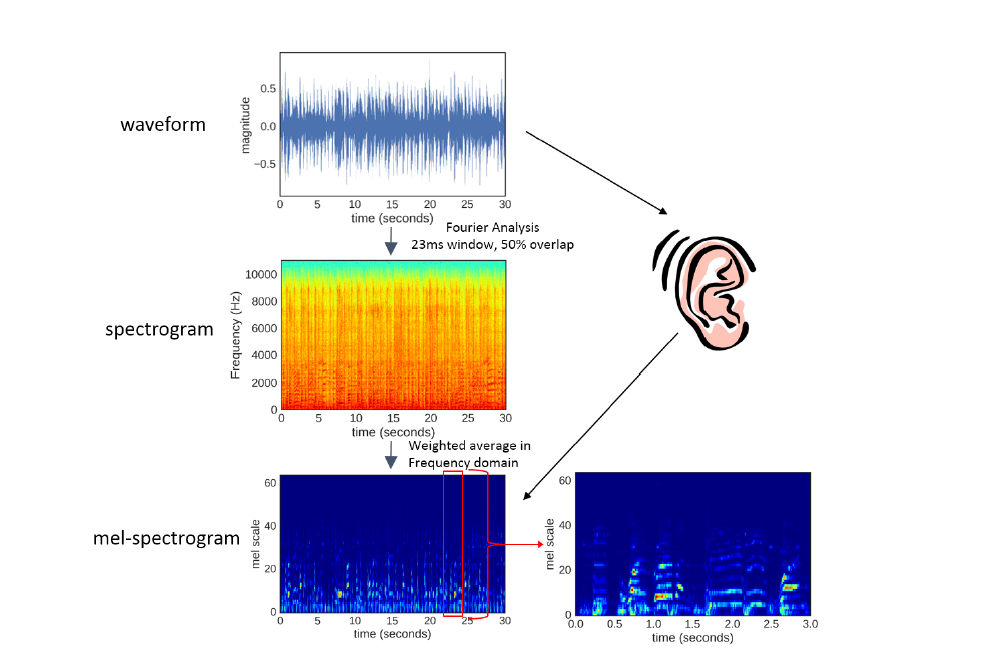
\includegraphics[scale=0.5]{./images/old-study/data-process.png}
		\caption{データ前処理}
		\label{fig:dataprocess}
		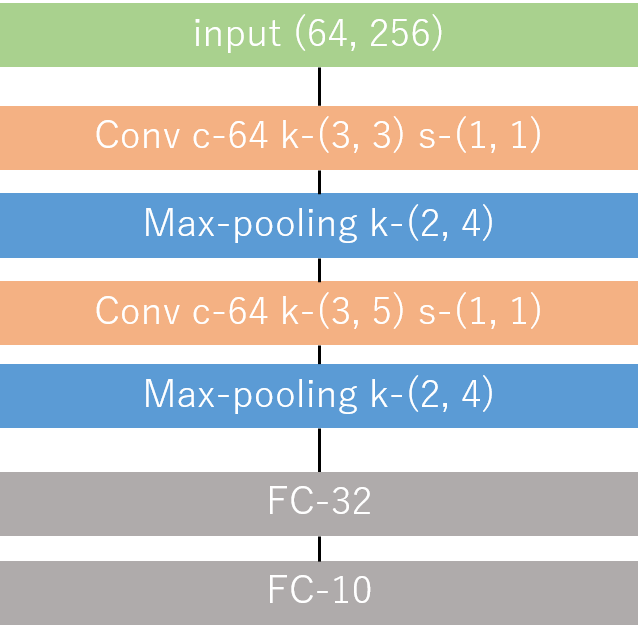
\includegraphics[scale=0.47]{./images/old-study/network.png}
		\caption{ネットワーク構成}
		\label{fig:mingwen-network}
	\end{center}
\end{figure}

\clearpage
\subsection{各ジャンルにおける分類精度}
ジャンル毎における分類精度を表した混同行列を\figref{fig:mingwen-table}に示す.\figref{fig:mingwen-table}から各ジャンルにおいて分類精度にばらつきがみられ,特にcountryとrockのジャンルにおいて精度が著しく低くなっている.
\begin{figure}[htbp]
	\begin{center}
		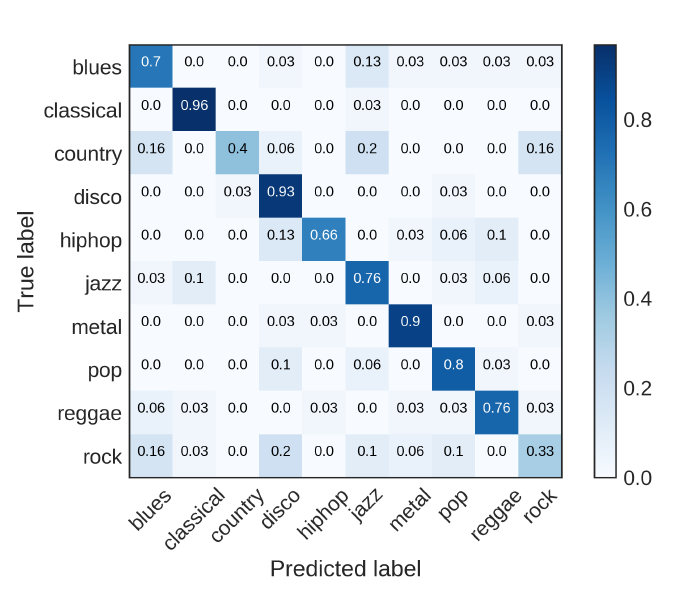
\includegraphics[scale=0.7]{./images/old-study/matrix.png}
		\caption{GTZANを用いた場合の各ジャンルにおける分類精度}
		\label{fig:mingwen-table}
	\end{center}
\end{figure}

\subsection{問題点}\label{cnn-problem}
初めに使用しているデータセットに問題点が挙げられ,GTZANデータセットは欠点が存在すると調査されている\cite{gtzanissue}.欠点の例として,ノイズしか鳴っていないデータがあったり,データセットに重複があるといったものがある.特に重複データにおいては異なるジャンル間で同じ楽曲データが存在してしまっている.そのため,テストデータに学習データが含まれてしまっている可能性があったり,ラベル付けが不適切であったりなど,実験結果の分類精度に信頼性と説得力が欠けている.


次にモデルの観点から見た問題点を述べる.これは学習済みモデルがブラックボックスなため,どういった点でジャンル分類しているかが不明であるということである.分類精度に改善の余地がみられる点から,モデルを修正する必要性があると考えられる.しかしながらジャンル間の境界面が不明瞭なことから,モデルをどのように修正すればよいのかという指標が立てにくく,試行錯誤的にネットワーク構成を変えながら実験するしかないのが現状である.

\section{Grad-CAM}
Grad-CAMは学習済みのCNNが画像を分類した際,画像のどの部分を強く見ているかをヒートマップ化する手法である\cite{gradcam}.

\subsection{入力画像のヒートマップ化}
Grad-CAMによる入力画像のヒートマップ化の全体の流れを\figref{fig:gradcam}に示す.
\begin{figure}[htbp]
	\begin{center}
		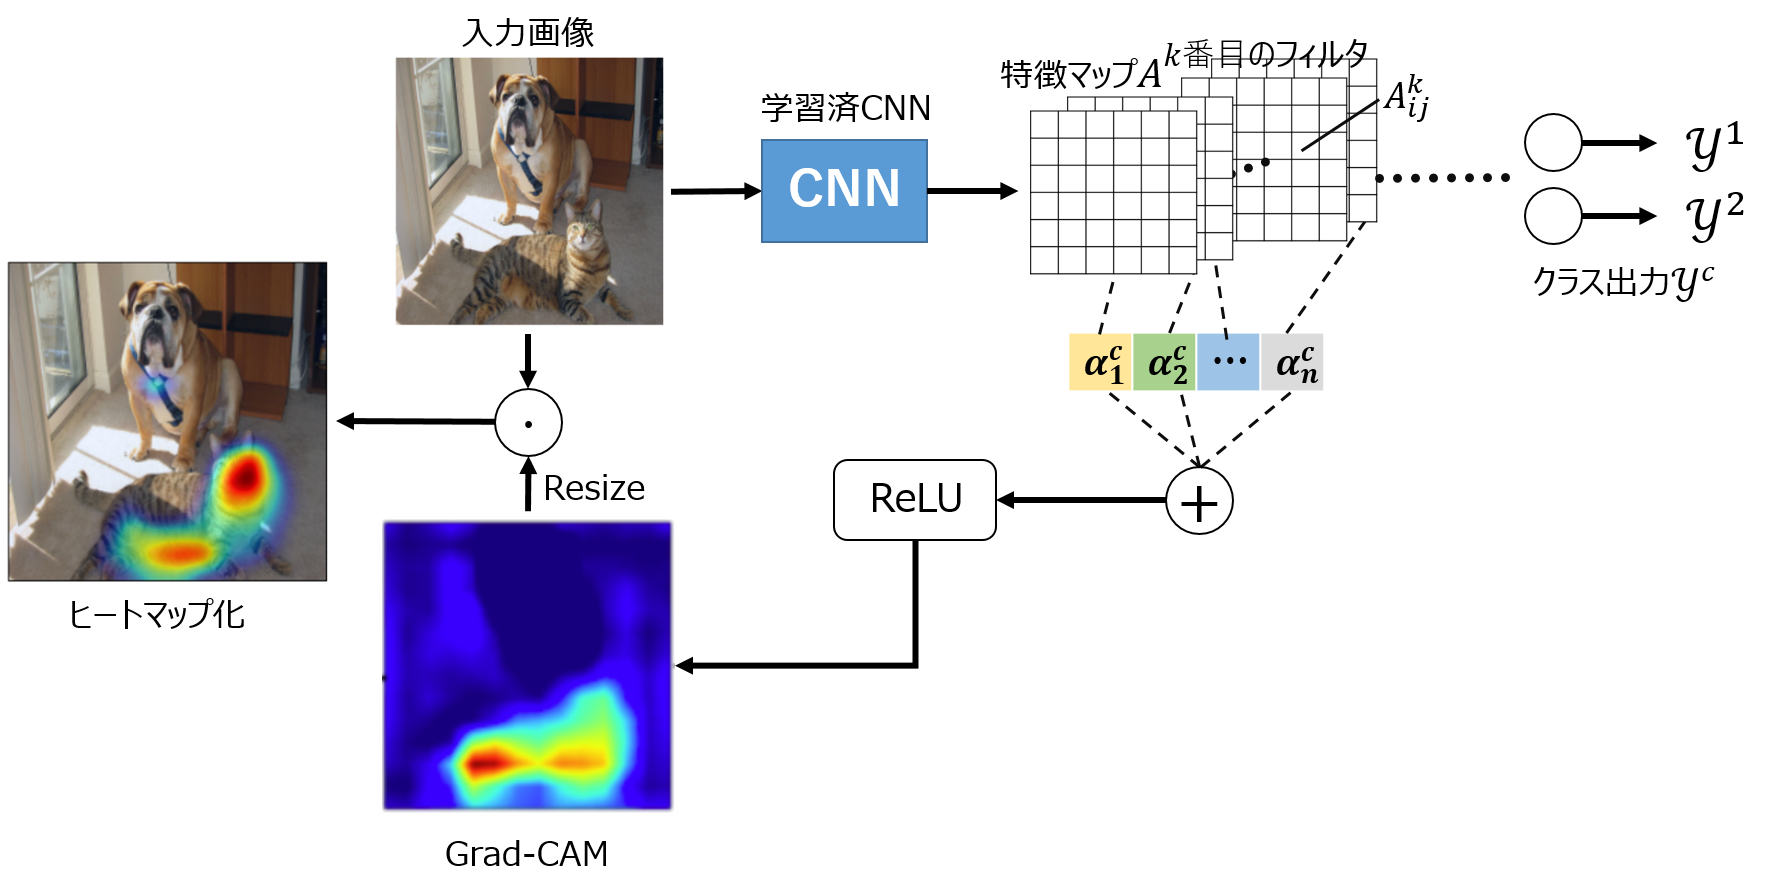
\includegraphics[scale=0.492]{./images/old-study/gradcam.png}
		\caption{Grad-CAMによるヒートマップ化}
		\label{fig:gradcam}
	\end{center}
\end{figure}

学習済みCNNに画像を入力したとき,畳み込み層で得られた$k$番目の特徴マップを$A^{k}_{ij}$,最終層で得られた$c$クラスの確率スコアを$y^c$とする.このとき\eref{eq:gradcam-weight}のように,確率スコアに対し特徴マップの勾配をとって平均化したものを重要度$\alpha^c_k$とする.
\begin{align}
	\alpha^c_k = \frac{1}{Z} \sum_i \sum_j \frac {\partial y^c}{\partial A^k_{ij}} \label{eq:gradcam-weight}
\end{align}
この$\alpha^c_k$を用いて,\eref{eq:gradcam-heatmap}で示すように$k$個の特徴マップで加重平均を計算し,活性化関数ReLUを通したものをヒートマップ出力として定義する.これは,$A^k_{ij}$の値の大きさに勾配の大きさも加味することでより重要な箇所を限定していることになる.
\begin{align}
	L^c_{Grad-CAM} = ReLU(\sum_k \alpha^c_k A^k) \label{eq:gradcam-heatmap}
\end{align}
最後にヒートマップを入力画像に合わせてリサイズし,入力画像との畳み込み演算により入力画像のヒートマップ化を行っている.


この手法の重要な点は$A^k_{ij}$の値をうごかした時に,$y^c$のスコアがどのように変化するかという点である.
$\frac {\partial y^c}{\partial A^k_{ij}} > 0$の場合は$A^k_{ij}$が増加する方向に$y^c$が増加し,$\frac {\partial y^c}{\partial A^k_{ij}} < 0$の場合は$A^k_{ij}$が減少する方向に$y^c$が増加する.このとき,$A^k_{ij}$はReLUを通した後の値と仮定すれば,$A^k_{ij} \geq 0$である.そのため,$\frac {\partial y^c}{\partial A^k_{ij}} < 0$の箇所は非活性なピクセルであると考えられ,\eref{eq:gradcam-heatmap}においてReLUを通すことで,勾配が正の部分だけでヒートマップ化を行っている.
\begin{figure}[htbp]
	\begin{center}
		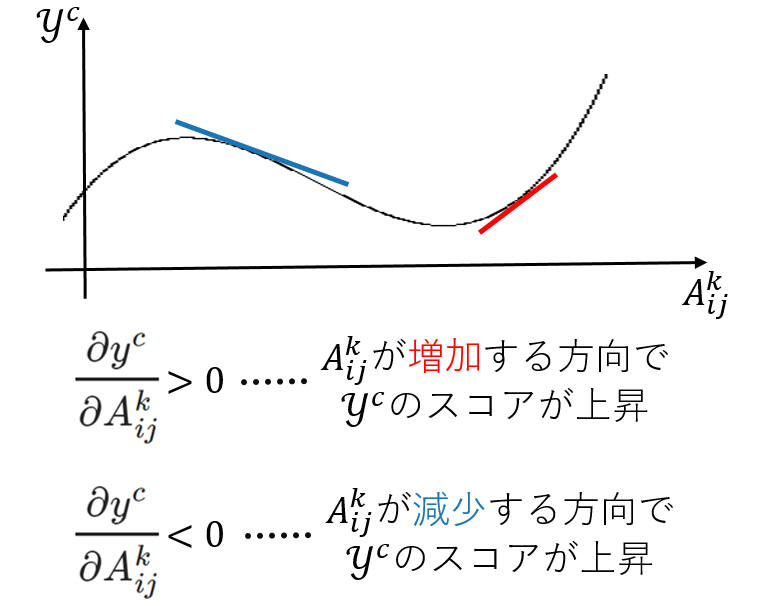
\includegraphics[scale=0.63]{./images/old-study/gradient.png}
		\caption{$A^k_{ij}$に関する勾配}
		\label{fig:featuremap-gradient}
	\end{center}
\end{figure}


\clearpage
\subsection{問題点}\label{gradcam-problem}
特徴マップによる勾配をとることから,ヒートマップの形が特徴マップのサイズや形に大きく依存してしまうという欠点がある.極端な例では,畳み込み後の特徴マップが$1\times 1$の場合ヒートマップ出力が$1\times 1$になってしまい,入力画像全体がヒートマップ化されてしまう.

また,勾配をとるという点で勾配消失の問題がある.例えば学習が十分に進んだモデルに対し,学習データに含まれる画像を入力した場合,$y_c$の確率スコアが限りなく1に近づく.この時ソフトマックス関数の勾配は限りなく0に近づくため,プログラム上で実装したとき勾配が0となってしまう.そのため重要度$\alpha^c_k$が0になってしまい,入力画像のヒートマップ化が不可能となる.


さらに,画像を入力としてクラス出力を行うため,画像を一枚一枚用意するのに手間がかかる.クラス間をまたがって画像は連続変化していくという前提を考えたとき,クラス境界となる画像が必ず存在する.しかし,その境界画像を確認するためには試行錯誤に画像を用意して探さなければならない.

\begin{figure}[htbp]
	\begin{center}
		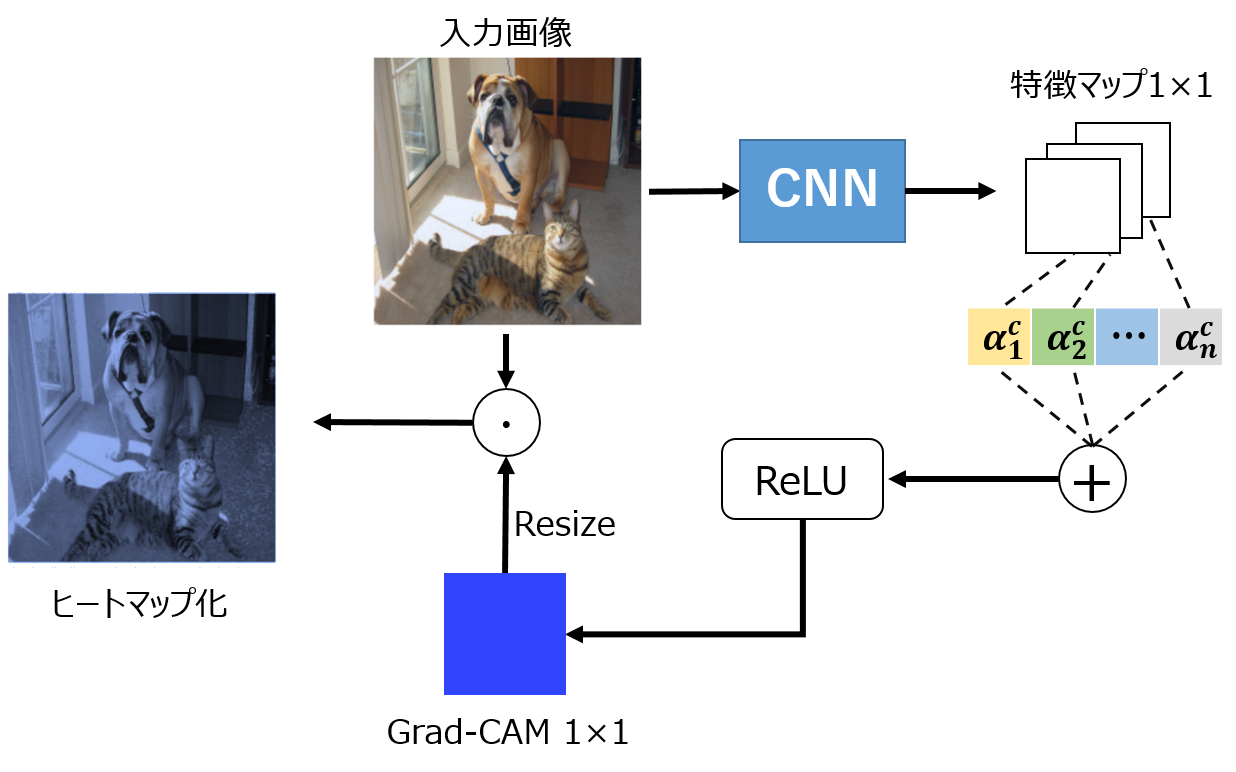
\includegraphics[scale=0.6]{./images/old-study/fail-gradcam.png}
		\caption{$1 \times 1$の特徴マップによるGrad-CAM}
	\end{center}
\end{figure}

\clearpage
\section{Harmonic/Percussive Separation using Median Filtering}
楽曲の周波数振幅スペクトログラムをメディアンフィルタを用いてハーモニー成分とパーカッション成分のスペクトログラムに分けた研究である\cite{percuss_harmony}.ハーモニー成分のスペクトログラムは周波数軸方向に表れ,パーカッション成分のスペクトログラムは時間軸方向に表れるという仮定のもと推定を行い,オリジナルのスペクトログラムにマスクすることによって一方の成分を取り出している.

\subsection{メディアンフィルタ}
メディアンフィルタは画像処理の分野で多く用いられており,主にノイズ除去のために使われている.メディアンはその名の通り中央値を表しており,\figref{fig:median-filter}のような1次元データがあったとき,値を小さい順に並べていき中央になった値をデータ配列の中心の値と置き換えるフィルタである.画像などといった2次元データの場合は\figref{fig:median-filter2}のようにフィルタの中央となる部分の値が置き換わる.

\begin{figure}[htbp]
	\begin{center}
		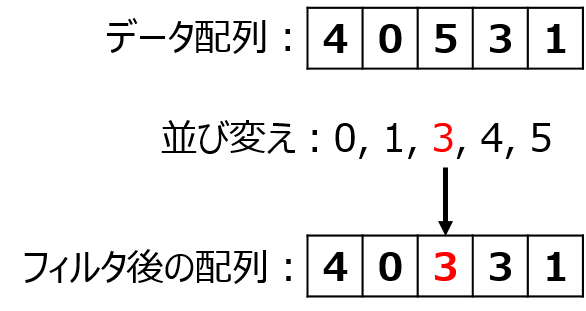
\includegraphics[scale=0.51]{./images/old-study/median-filter.png}
		\caption{1次元メディアフィルタの動作}
		\label{fig:median-filter}		
	\end{center}
\end{figure}

\begin{figure}[htbp]
	\begin{center}
		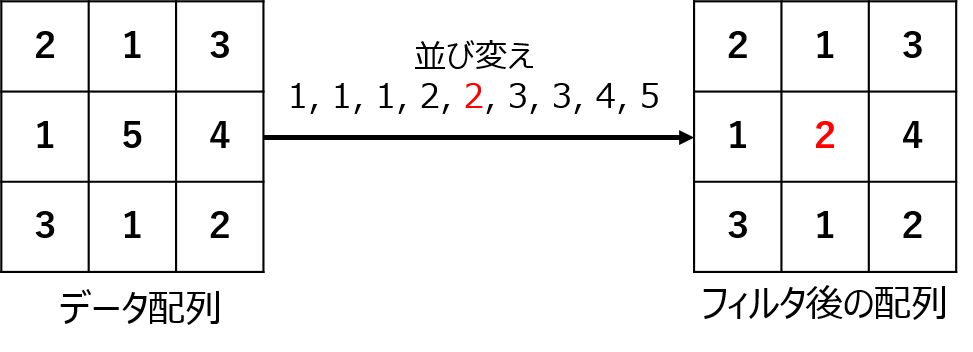
\includegraphics[scale=0.5]{./images/old-study/median-filter2.png}
		\caption{2次元メディアフィルタの動作}
		\label{fig:median-filter2}
	\end{center}
\end{figure}


\subsection{ハーモニー成分とパーカッション成分}
ハーモニー成分のスペクトログラムは周波数軸方向に表れやすいと仮定する.この仮定により,周波数軸方向にメディアンフィルタを適用していけばハーモニー成分を取り除くことができる.\figref{fig:median-fre}上はスネアとピアノがミックスされた音の特定時間におけるスペクトラムであり,\figref{fig:median-fre}下は周波数軸方向にメディアンフィルタを掛けた後のスペクトラムである.
\figref{fig:median-fre}より,ピアノのハーモニーの主となるスペクトラムの倍音のピークがメディアンフィルタによって消えていることから,メディアンフィルタはハーモニー成分を取り除いていることが分かる.
\begin{figure}[htbp]
	\begin{center}
		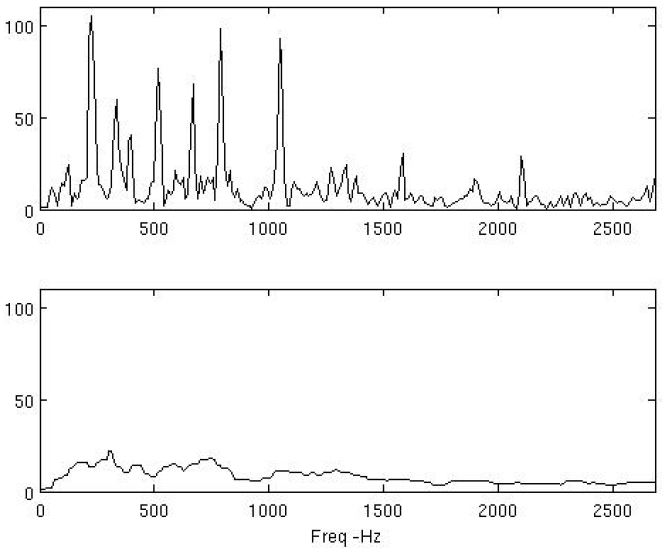
\includegraphics[scale=0.363]{./images/old-study/median-fre.png}
		\caption{周波数軸に対するメディアンフィルタ}
		\label{fig:median-fre}
	\end{center}
\end{figure}


次に,パーカッション成分は時間軸方向のオンセットに表れやすいと仮定する.同様に,時間軸方向にメディアンフィルタを適用していけばパーカッション成分を取り除くことができる.\figref{fig:median-time}上はスネアとピアノがミックスされた音の特定周波数における時間軸の増減を表してており,\figref{fig:median-time}下は時間軸方向にメディアンフィルタを掛けた後の特定周波数における時間軸の増減である.
\figref{fig:median-time}より,スネアの主となるオンセットがメディアンフィルタによって抑制されているため,パーカッション成分を取り除いていることが分かる.

\begin{figure}[htbp]
	\begin{center}
		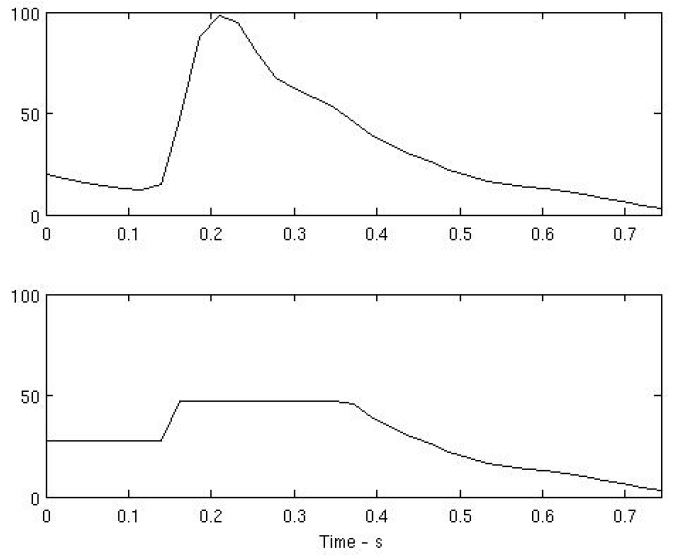
\includegraphics[scale=0.363]{./images/old-study/median-time.png}
		\caption{時間軸に対するメディアンフィルタ}
		\label{fig:median-time}
	\end{center}
\end{figure}


\subsection{ハーモニー成分とパーカッション成分の分離}
楽曲のスペクトログラムをハーモニー成分とパーカッション成分に分離することを考える.
楽曲信号をフーリエ変換して得られたスペクトログラムを,周波数軸方向を$h$と時間軸方向を$i$として$S_{h,i}$と表し,ハーモニー成分が抑制されたのスペクトログラムを$H_{h, i}$,パーカッション成分が抑制されたスペクトログラムを$P_{h, i}$とすると,\eref{eq:har},\eref{eq:per}が成り立つ.
\begin{eqnarray}
	H_{h, i} = {\rm MF} (S_h, l_h) \label{eq:har}\\
	P_{h, i} = {\rm MF} (S_i, l_i) \label{eq:per}
\end{eqnarray}
MFはメディアンフィルタを示し,$l_h, l_i$はそれぞれフィルタの長さとする.この$H_{h, i}, P_{h, i}$を用いて\eref{eq:mask-h}, \eref{eq:mask-p}もしくは\eref{eq:mask-h2}, \eref{eq:mask-p2}のようにして,ハーモニー成分のマスクスペクトログラム$M_{H_{h, i}}$とパーカッション成分のマスクスペクトログラム$M_{P_{h, i}}$を作成する.

\clearpage
\begin{eqnarray}
	M_{H_{h, i}} &=& \begin{cases}
		1 & (H_{h, i} > P{h, i})\\
		0 & (otherwise)
		\end{cases} \label{eq:mask-h} \\
	M_{P_{h, i}} &=& \begin{cases}
		1 & (P_{h, i} > H{h, i})\\
		0 & (otherwise)
		\end{cases}\label{eq:mask-p} \\
	M_{H_{h, i}} &=& \frac{H^k_{h, i}}{H^k_{h, i} + P^k_{h, i}} \label{eq:mask-h2} \\
	M_{H_{h, i}} &=& \frac{P^k_{h, i}}{H^k_{h, i} + P^k_{h, i}} \label{eq:mask-p2}
\end{eqnarray}
\eref{eq:mask-h2}, \eref{eq:mask-p2}における$k$は1か2の値をとる.\\
最後に\eref{eq:gen-har}, \eref{eq:gen-per}のように,得られたマスクスペクトログラムをオリジナルのスペクトログラムに畳み込みこむことでハーモニー成分$\hat{\rm \bf H}$とパーカッション成分$\hat{\rm \bf P}$を得る.
\begin{eqnarray}
	\hat{\rm \bf H} = \hat{\rm \bf S} \otimes \rm \bf M_H \label{eq:gen-har} \\
	\hat{\rm \bf P} = \hat{\rm \bf S} \otimes \rm \bf M_P \label{eq:gen-per}
\end{eqnarray}

\subsection{メリット}
メディアンフィルタという特定のフィルタを用いていることから,検出方法が自明である.そのため成分を分ける操作において,機械学習などを用いたときに現われるブラックボックスといった問題点がないということが良い点であると言える.また,アルゴリズムが比較的容易なため,プログラムの実装が簡単であり,さらにはライブラリ等でも実装されている.また,パーカッション成分とハーモニー成分をマスクするデータを作る際に,それぞれの成分で仮定した定義が直感的にも当てはまる.以上の点から本研究で楽曲データセットに対し,ハーモニー成分とパーカッション成分を分ける際に使用する.
